Setup which is used in this research paper is very simple. There are
actually two setups, because there were a need to record cloud
coverage data from somewhere, and at the same time there were a need
to record solar panel data.

First setup which collects solar panel data is placed in a town named
Mønsted which can be seen on a picture below. The setup consists of
PV, inverter, and raspberry pi, which collects data into a SQL
database.

The second setup which records cloud coverage data is placed inside
Aarhus university, where a stationary computer is running and
gathering data from OpenWeather.com api, and stores the data into
separate sql database. Data which is gathered from OpenWeather api are
coming from two different towns Stoholm and Karup where both towns are
closest to first setups placement, and there are no way to force
OpenWeather api to return data from the same town always.

At last data from both setups are read into one main DB where data
gets treated.

\begin{figure}[h]
  \centering
 % 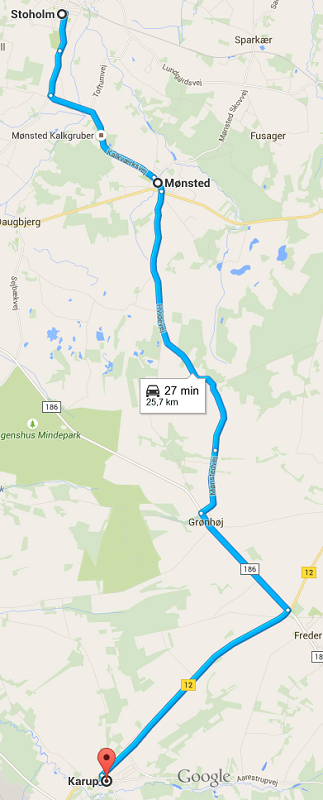
\includegraphics{MapsPicture.png}
 
\includegraphics{dummy.jpg}
  \caption{3 towns where data is recorded}
      \label{fig:MapsPicture}
\end{figure}